\section{Analysis}
\subsection{Problem Defenition}
The goal of this project is to design the hardware specification for a custom 16-bit single cycle CPU, and develop the suite of tools required to simulate such a processor, including an Emulator (\ref{sec:Emulator}), Assembler (\ref{sec:Assembler}), and Compiler (\ref{sec:Compiler}). The project will detail the abstract design of the computer’s Instruction Set Architecture (ISA) (\ref{sec:ISA}) and its implementation in hardware, considering the internal registers, system clock, main memory, and fetch execute cycle.

The project will compose three primary parts, an emulator capable of loading machine code 'catridges' and simulating the hardware, memory, peripherals and registers detailed by the ISA in order to execute programs with correct clock timing and behaviour. An assembler to translate programs written in an assembly specification into binary machine code (the assembler will handle higher level conveniences such as relative addressing through labels). And finally a compiler - to translate a higher level programming langauge into machine code. This will require compiler optimisations with relation to the produced object code; complex data structures such as arrays, objects and strings; conditional and interative expressions; and functions and procedures. The suite required to simulate such a computer should be capeable of writing and compiling complex programs such as pong or tetris, and emulating them with hardware correct timings - dealing with peripherals such as a keyboard or speaker.

\subsection{Background to the Problem Area}
This project will explore lower level systems software and look in detail at the fundemental architecture of modern computing systems and how they are designed from the ground up.

\subsubsection{Instruction Set Architecture}
\label{sec:ISA}
The ISA acts as an interface between the hardware and software of a computing system, and contains crucial information regarding the capabilities of a processor, including: a functional defenition of storage locations (e.g. registers and memories) as well as a description of all instructions and operations supported.

An ISA can be classified according to its architectural comlpexity into a Complex Instruction Set Computer (CISC), or a Reduced Instruction Set Computer (RISC). A CISC processor implements a wide variety of specialized instructions in hardware (e.g. floating point arithmetic or transferring multiple registers to or from the stack), minimising the number of instructions per program at the cost of a more complex design, higher power consumption and slower execution as each instruction requires more processor cycles to complete. \textcite{gfg-risc-vs-cisc} Thus optimisations in performance occur on the hardware level. This is historically the most common branch of processor and often results in processors with large instruction sets, for example the Intel x86's 1503 defined instructions \textcite{ryg-blog}. A RISC processor however aims to simplify hardware using an instruction set consisting of a few basic instructions to load, evaluate and store data - instead placing optimisations on the software side unlike a CISC processor. This has the side effect of increased memory usage required to store additional instructions needed to perform complex tasks.

\subsubsection{Emulator}
\label{sec:Emulator}
An emulator is a software program that allows one computer to imitate another - and by simulating the hardware of the other – execute machine code programs written for a processor other than itself. Emulators tend to consist of three modules, a CPU emulator, memory subsystem module, and I/O device emulators \textcite{retroreversing}. The simplest form of CPU emulator is an interpreter - wherein the emulator steps sequentially through each machine code instruction, and carries out the fetch-decode-execute cycle for each, modifying the internal state of the simulated processor in the same manner as the instruction would affect the physical hardware - this can be achieved by representing internal flags and registers as variables. The Memory Subsystem can be implemented as a one dimensional array of bytes - with features such as memory mapped I/O implemented by associating regions of memory to peripherals and subsystems, e.g. Video Random Access Memory (VRAM), the stack, and the heap. 

\subsubsection{Assembler}
\label{sec:Assembler}
An assembler is a program that translates assembly language (a low level programming language that uses mneumonics to directly represent machine code instructions) into object code that can be executed by the processor. 

\subsubsection{Compiler}
\label{sec:Compiler}
A compiler is a program that translates high level program source code into a set of machine language instructions. Some compilers translate source code into an intermediate assembly language before using an assembler to produce the machine code instructions, whereas others compile into machine code directly.

\subsection{Programming Language}
\subsection{Existing Systems}
\subsubsection{The Hack Computer}
\subsubsection{University of Washington MIPS Computer}
The following system is a 16 bit MISC (Minimal Instruction Set Computer) processor designed by the University of Washington for a series of lectures as part of their computer science course \textcite{MIPS-uw}. A MISC processsor is a subclass of the RISC processor and involves minimising the number of instructions implemented in hardware, resulting in far simpler hardware designs - where a RISC processor may have 30-70 instructions, a MISC processor may have merely 10-20 consisting of arithmetic, branching, loading and storing instructions. \textcite{MISC-dakeng}. 

A MIPS (Microprocessor without Interlocked Pipelined Stages) processor such as this does not overlap the execution of several instructions (pipelining), thus neglecting the potential performance gains in favor of a simpler architecture. This processor is a single-cycle implementation meaning all instructions take exactly one cycle to complete, this is achieved using a Harvard architecture in place of Von Neuman wherein instructions are stored in a seperate Read Only Memory (ROM) to data, thus both can be fetched within the same processor cycle. 

The processor supports the following instructions:
\begin{enumerate}
    \item Arithmetic \texttt{add, sub, and, or, slt (set if less than)}
    \item Data Transfer \texttt{lw (load word), sw (store word)}
    \item Control \texttt{beq (branch if equal to)}
\end{enumerate} 
Register-to-Register arithmetic instructions use the R-type encoding for their machine code representation, where \texttt{op} is the opcode of the instruction with \texttt{func} representing the particular arithmetic operation. \texttt{rs, rt}, and \texttt{rd} are the source and destination registers. This computer operates on an ALU with a 3 bit control signal supporting 5 operations that directly correspond to the \texttt{func} portion of an R type instructions binary encoding. 

\bigskip

\shadowbox{
    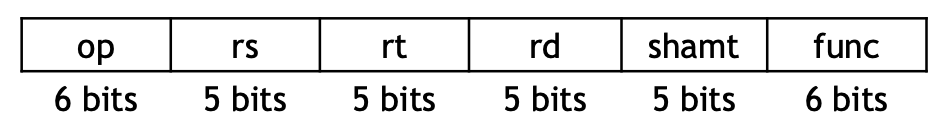
\includegraphics[width=11cm]{Screenshot 2024-04-14 at 22.19.47.png}
}

\bigskip

The I type encoding is the second means for which instructions can be represented, and includes the data transfer and control instructions \texttt{lw, sw}, and \texttt{beq} specified above. \texttt{address} is a signed 16 bit constant. \texttt{rt} is the destination for \texttt{lw} and source for \texttt{beq} and \texttt{sw}. \texttt{rs} is the base register for the \texttt{lw} and \texttt{sw} instructions (added to the sign extended constant \texttt{address} to get a data memory address) \textcite{MIPS-uw}. In this processor design, for a \texttt{beq} instruction, the \texttt{address} field specifies not a memory address, rather a signed offset from which to jump from the current PC position when executing the branch instruction.

\bigskip

\shadowbox{
    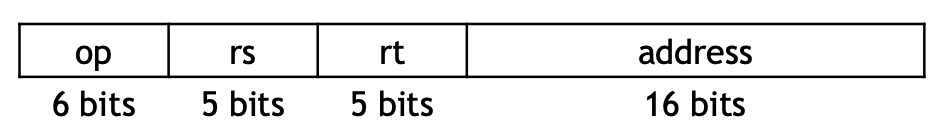
\includegraphics[width=11cm]{Screenshot 2024-04-14 at 22.33.16.png}
}

\bigskip

Below is the full datapath specification for the computer, with the Instruction Memory (ROM) on the left, connected to the PC in order to address instructions. Those instructions are in turn passed through the control unit and decoded, with the opcode specifying whether an I or R type instruction is being processed and accordingly what hardware should be used to interpret and execute the instruction. This dictates the calculation (if any) that is to be performed in the ALU - the output of which is stored in a seperate data memory.

Since instructions are stored in a seperate ROM, the address of the first instruction will always begin at 0 - this simplifies the calculation of offsets and labels in the assembler – since the assumption that the first instruction begins at address 0 will always hold true. However, branch instructions are handled unusually in this computer - instead of specifying the jump address, the signed offset from the current instruction is specified instead. This has the effect of making compilation easier as branch addresses do not need to be calculated by the assembler, however renders specific jumps to memory addresses (such as the location of an interrupt service routine or bootloader) difficult.

\bigskip

\shadowbox{
    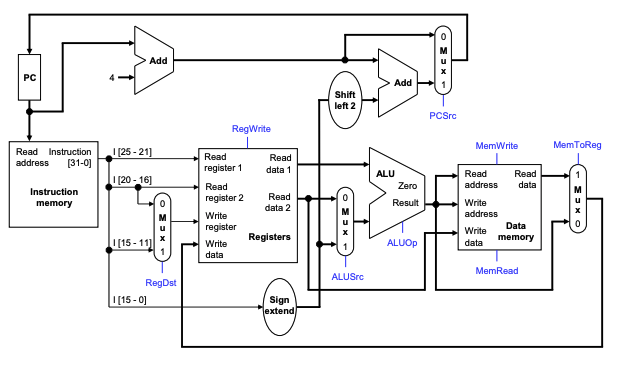
\includegraphics[width=11cm]{Screenshot 2024-04-14 at 19.42.11.png}
}

The architecture described above has some notable advantages, firstly, its Harvard architecture allows the processor to operate each instruction in a single cycle – both improving performance and simplifying the design of the emulator as microinstruction cycles do not need to be simulated  to accurately simulate the hardware. Secondly, by dividing the computer architecture into 2 distinct I and R type instructions, you can reduce redundant information – and thus the bits required to store machine code instructions and programs.

However, this simple architecture results in many inconveniences when writing assembly code - due to the limited instruction set, simple tasks take comparatively more instructions meaning programs are longer and more tedious to write - as well utilising more memory due to the limited number of specialized instructions who's functionality must be implemented using handwritten subroutines such as binary shifts, stack operations, or interrupt handling. 

\bigskip

The takeaways of this system for my project include:
\begin{enumerate}
    \item The encoding of instructions into meaningful machine code that directly relates to the hardware of the computer - for instance R type opcodes representing the control bits of the ALU, this makes decoding instructions more efficient - especially when implmented in hardware.
    \item Secondly, the behaviour of hardware (registers, memories, flags) and the relationships between components during a single-cycle Harvard fetch-execute cycle that will have to be simulated when designing an emulator.
    \item I will also expand the instruction set further than the MISC specification used in this processor to include other common instructions, and keep the memory-register seperation wherin operations are performed on register values, with 2 instructions \texttt{lw, sw} used for reading and writing to memory.
    \item I will also change the branch instruction to operate on absolute addresses rather than signed offsets.
\end{enumerate}

\subsection{Prototyping}
\subsection{Client Proposal}
\subsubsection{Client Interview}
\subsection{Objectives}